\subsection{两个根之间的关系}

回顾一下，从现在起我们假设 k = R。（将定义和结果推广到一般情形的任务留给读者，方法见第 1 号的注记 2。）

以下始终，R 表示向量空间 V 中的一个根系；并且 V 配备了一个在 W(R) 下不变的内积 \((x,y)\mapsto(x|y)\)，cf.~Prop. 3。

设 \(\alpha, \beta \in \mathbb{R}\)。由第 1 号的公式 (7)，

\[
n (\alpha , \beta) n (\beta , \alpha) = 4 \cos^ {2} (\widehat {\alpha , \beta}) \leqslant 4.\tag{10}
\]

因此，整数 \(n(\alpha,\beta)n(\beta,\alpha)\) 必须取 0、1、2、3、4 中的一个值。根据 Chap. V, § 2, no. 5 的 Prop. 6 的 Cor. 以及 Chap. V, § 4, no. 8 页上的脚注，我们看到，除交换 \(\alpha\) 与 \(\beta\) 外，唯一的可能性如下：

\[
1) \quad n (\alpha , \beta) = n (\beta , \alpha) = 0; \quad \widehat {(\alpha , \beta)} = \frac {\pi}{2}; \quad s _ {\alpha} s _ {\beta} \text {of order} 2;
\]

\[
2) \quad n (\alpha , \beta) = n (\beta , \alpha) = 1; \quad (\alpha , \beta) = \frac {\pi}{3}; \quad s _ {\alpha} s _ {\beta} \text {   of   order   } 3;
\]

\[
\parallel \alpha \parallel = \parallel \beta \parallel ;
\]

\[
3) \quad n (\alpha , \beta) = n (\beta , \alpha) = - 1;
\]

\[
\widehat {(\alpha , \beta)} = \frac {2 \pi}{3};
\]

\[
s _ {\alpha} s _ {\beta} \text {of order 3};
\]

\[
\| \alpha \| = \| \beta \|;
\]

\[
4) \quad n (\alpha , \beta) = 1, n (\beta , \alpha) = 2; \qquad \widehat {(\alpha , \beta)} = \frac {\pi}{4};
\]

\[
s _ {\alpha} s _ {\beta} \text {   of   order   4;   }
\]

\[
\parallel \beta \parallel = \sqrt {2} \parallel \alpha \parallel ;
\]

\[
5) \quad n (\alpha , \beta) = - 1, n (\beta , \alpha) = - 2;
\]

\[
\widehat {(\alpha , \beta)} = \frac {3 \pi}{4};
\]

\[
s _ {\alpha} s _ {\beta} \text {   of   order   4;   }
\]

\[
\parallel \beta \parallel = \sqrt {2} \parallel \alpha \parallel ;
\]

\[
6) \quad n (\alpha , \beta) = 1, n (\beta , \alpha) = 3;
\]

\[
\widehat {(\alpha , \beta)} = \frac {\pi}{6};
\]

\[
s _ {\alpha} s _ {\beta} \text {   of   order   } 6;
\]

\[
\parallel \beta \parallel = \sqrt {3} \parallel \alpha \parallel ;
\]

\[
7) \quad n (\alpha , \beta) = - 1, n (\beta , \alpha) = - 3;
\]

\[
\widehat {(\alpha , \beta)} = \frac {5 \pi}{6};
\]

\[
s _ {\alpha} s _ {\beta} \text {   of   order   6;   }
\]

\[
\parallel \beta \parallel = \sqrt {3} \parallel \alpha \parallel ;
\]

\begin{enumerate}
\def\labelenumi{\arabic{enumi})}
\setcounter{enumi}{7}
\item
  \(n(\alpha, \beta) = n(\beta, \alpha) = 2; \quad \alpha = \beta;\)
\item
  \(n(\alpha, \beta) = n(\beta, \alpha) = -2; \quad \alpha = -\beta;\)
\item
  \(n(\alpha, \beta) = 1\) , \(n(\beta, \alpha) = 4\) ; \(\beta = 2\alpha\) ;
\item
  \(n(\alpha, \beta) = -1\) , \(n(\beta, \alpha) = -4\) ; \(\beta = -2\alpha\) .
\end{enumerate}

特别地：

命题 8. (i) 若两个根成比例，则比例因子只能是 \(\pm 1, \pm \frac{1}{2}, \pm 2\)。

\begin{enumerate}
\def\labelenumi{(\roman{enumi})}
\setcounter{enumi}{1}
\tightlist
\item
  若 \(\alpha\) 和 \(\beta\) 是两个不成比例的根，且 \(\| \alpha \| \leqslant \| \beta \|\)，则 \(n(\alpha, \beta)\) 取 \(0, 1, -1\) 中的一个值。
\end{enumerate}

若根 \(\alpha \in \mathbb{R}\) 满足 \(\frac{1}{2}\alpha \notin \mathbb{R}\)，则称 \(\alpha\) 为不可分根。

定理 1. 设 \(\alpha, \beta\) 是两个根。

\begin{enumerate}
\def\labelenumi{(\roman{enumi})}
\item
  若 \(n(\alpha, \beta) > 0\)，则 \(\alpha - \beta\) 是根，除非 \(\alpha = \beta\)。
\item
  若 \(n(\alpha, \beta) < 0\)，则 \(\alpha + \beta\) 是根，除非 \(\alpha = -\beta\)。
\end{enumerate}

若 \(n(\alpha, \beta) > 0\)，则根据上面的列表，可能性如下：

\begin{enumerate}
\def\labelenumi{\arabic{enumi})}
\item
  \(n(\alpha, \beta) = 1\)；于是 \(\alpha - \beta - s_{\beta}(\alpha) \in \mathbb{R}\)；
\item
  \(n(\beta, \alpha) = 1\)；于是 \(\beta - \alpha = s_{\alpha}(\beta) \in \mathbb{R}\)，所以 \(\alpha - \beta \in \mathbb{R}\)；
\item
  \(\beta = \alpha\) .
\end{enumerate}

这证明了 (i)，而 (ii) 由将 \(\beta\) 换成 \(-\beta\) 得到。

推论。设 \(\alpha\) 和 \(\beta\) 是两个根。

\begin{enumerate}
\def\labelenumi{(\roman{enumi})}
\item
  若 \((\alpha |\beta) > 0\)，则 \(\alpha - \beta\) 是根，除非 \(\alpha = \beta\)。
\item
  若 \((\alpha |\beta) < 0\)，则 \(\alpha + \beta\) 是根，除非 \(\alpha = -\beta\)。
\item
  若 \(\alpha - \beta \notin R \cup \{0\}\) 且 \(\alpha + \beta \notin R \cup \{0\}\)，则 \((\alpha | \beta) = 0\)。
\end{enumerate}

断言 (i) 和 (ii) 由 Th. 1 以及第 1 号的公式 (7) 得到。断言 (iii) 由 (i) 和 (ii) 得到。

可能有 \(\alpha + \beta \in \mathbb{R}\) 且 \((\alpha|\beta) = 0\)（cf.~Plate X, System \(B_{2}\)）。当 \(\alpha - \beta \notin \mathbb{R} \cup \{0\}\) 且 \(\alpha + \beta \notin \mathbb{R} \cup \{0\}\) 时，称 \(\alpha\) 与 \(\beta\) 强正交。

命题 9. 设 \(\alpha\) 和 \(\beta\) 是两个不成比例的根。

\begin{enumerate}
\def\labelenumi{(\roman{enumi})}
\item
  整数 \(j\) 的集合 I（使得 \(\beta + j\alpha\) 是根）是包含 0 的区间 \([-q, p]\)，位于 \(\mathbf{Z}\) 中。
\item
  设 \(S\) 是由 \(\beta + j\alpha\)（其中 \(j \in I\)）组成的集合。于是，
\end{enumerate}

\[
s _ {\alpha} (S) = S \text { and } s _ {\alpha} (\beta + p \alpha) = \beta - q \alpha .
\]

\begin{enumerate}
\def\labelenumi{(\roman{enumi})}
\setcounter{enumi}{2}
\tightlist
\item
  \(p - q = -n(\beta, \alpha)\)。
\end{enumerate}

显然，\(0 \in I\)。设 \(p\)（相应地，\(-q\)）是 \(I\) 的最大（相应地，最小）元素。若不是区间 \([-q, p]\) 中的所有整数都属于 \(I\)，则存在两个整数 \(r, s\) 在区间 \([-q, p]\) 中，具有以下性质：\(s > r + 1\)、\(s \in I\)、\(r \in I\)，并且 \(r + k \notin I\) 对 \(1 \leqslant k \leqslant s - r - 1\) 成立。按照 Th. 1 的 Cor. 的记号，有 \((\alpha|\beta + s\alpha) \leqslant 0\)、\((\alpha|\beta + r\alpha) \geqslant 0\)，这不可能，因为

\[
(\alpha | \beta + s \alpha) \leqslant 0 > (\alpha | \beta + r \alpha).
\]

这证明了 (i)。

我们有 \(s_{\alpha}(\beta + j\alpha) = \beta - n(\beta, \alpha)\alpha - j\alpha = \beta + j'\alpha\)，其中 \(j' = -j - n(\beta, \alpha)\)。因此 \(s_{\alpha}(S) \subseteq S\)，从而 \(s_{\alpha}(S) = S\)。现在 \(j \mapsto -j - n(\beta, \alpha)\) 是从 I 到 I 的递减双射。于是，\(j' = -q\) 在 \(j = p\) 时成立，从而 \(-q = -p - n(\beta, \alpha)\)。这证明了 (ii) 和 (iii)。

集合 S 称为 \(\alpha\)-根链，它由 \(\beta\) 定义；\(\beta - q\alpha\) 是其起点，\(\beta + p\alpha\) 是其终点，而 \(p + q\) 是其长度。

推论。设 S 是根的 \(\alpha\)-链，\(\gamma\) 是 S 的起点。S 的长度为 \(-n(\gamma,\alpha)\)；它等于 0、1、2 或 3。

第一个断言由将 \(\beta = \gamma\) 应用于命题 9 的 (iii)，并利用 \(q = 0\) 这一事实得到。

另一方面，由于 \(\gamma\) 与 \(\alpha\) 不成比例，本号开头给出的列表表明 \(|n(\gamma,\alpha)|\leqslant3\)，故得出该推论。

注。沿用上述记号。则：

\begin{enumerate}
\def\labelenumi{\arabic{enumi})}
\item
  若 S 的长度为 0，则 \((\alpha |\gamma) = 0\)。
\item
  若 \(S\) 的长度为 1，则 \(n(\gamma, \alpha) = -1\)，且有三种情形：
\end{enumerate}

\[
n (\alpha , \gamma) = - 1, \quad (\alpha | \alpha) = (\gamma | \gamma), \quad (\alpha | \gamma) = - \frac {1}{2} (\alpha | \alpha), \quad \widehat {(\alpha , \gamma)} = \frac {2 \pi}{3}
\]

\[
n (\alpha , \gamma) = - 2, \quad (\alpha | \alpha) = 2 (\gamma | \gamma), \quad (\alpha | \gamma) = - \frac {1}{2} (\alpha | \alpha), \quad \widehat {(\alpha , \gamma)} = \frac {3 \pi}{4}
\]

\[
n (\alpha , \gamma) = - 3, \quad (\alpha | \alpha) = 3 (\gamma | \gamma), \quad (\alpha | \gamma) = - \frac {1}{2} (\alpha | \alpha), \quad (\widehat {\alpha , \gamma}) = \frac {5 \pi}{6}
\]

\pandocbounded{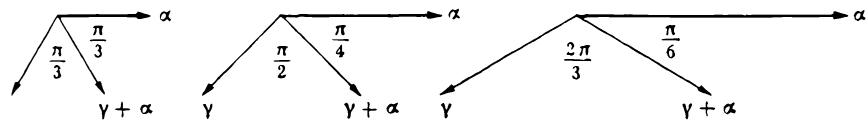
\includegraphics[keepaspectratio]{images/part001_d4d2d336.jpg}}

\begin{enumerate}
\def\labelenumi{\arabic{enumi})}
\setcounter{enumi}{2}
\tightlist
\item
  若 \(S\) 的长度为 2，则 \(n(\gamma, \alpha) = -2\)，因此
\end{enumerate}

\[
n (\alpha , \gamma) = - 1, (\alpha | \alpha) = \frac {1}{2} (\gamma | \gamma), (\alpha | \gamma) = - (\alpha | \alpha), \widehat {(\alpha , \gamma)} = \frac {3 \pi}{4}.
\]

\pandocbounded{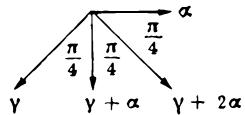
\includegraphics[keepaspectratio]{images/part001_f07fa75a.jpg}}

\begin{enumerate}
\def\labelenumi{\arabic{enumi})}
\setcounter{enumi}{3}
\tightlist
\item
  若 \(S\) 的长度为 3，则 \(n(\gamma, \alpha) = -3\)，因此
\end{enumerate}

\[
n (\alpha , \gamma) = - 1, (\alpha | \alpha) = \frac {1}{3} (\gamma | \gamma), (\alpha | \gamma) = - \frac {3}{2} (\alpha | \alpha), (\widehat {\alpha , \gamma}) = \frac {5 \pi}{6}.
\]

\pandocbounded{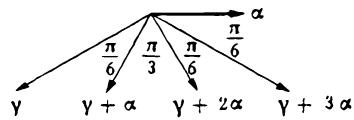
\includegraphics[keepaspectratio]{images/part001_9d247bec.jpg}}

我们将看到（Plate X, Systems \(A_{2}, B_{2}, G_{2}\)），所有这些情形实际上都能实现。

命题 10. 设 \(\alpha, \beta\) 是两个不成比例的根，且 \(\beta + \alpha\) 是一个根。设 \(p, q\) 是命题 9 中的整数。则

\[
\frac {(\beta + \alpha | \beta + \alpha)}{(\beta | \beta)} = \frac {q + 1}{p}.
\]

设 \(S\) 是 \(\alpha\)-链，由 \(\beta\) 定义，\(\gamma\) 是其起点；其长度 \(l\) 满足 \(\geqslant 1\)，因为 \(\beta + \alpha\) 是根。可能的情形如下：

\begin{enumerate}
\def\labelenumi{\arabic{enumi})}
\item
  \(l = 1\)；于是 \(\beta = \gamma, q = 0, p = 1, (\beta + \alpha | \beta + \alpha) = (\beta | \beta)\)。
\item
  \(l = 2\)，\(\beta = \gamma\)；于是 \(q = 0\)，\(p = 2\)，\((\beta + \alpha|\beta + \alpha) = \frac{1}{2} (\beta|\beta)\)。
\item
  \(l = 2, \beta = \gamma + \alpha\)；于是 \(q = 1, p = 1, (\beta + \alpha|\beta + \alpha) = 2(\beta|\beta)\)。
\item
  \(l = 3, \beta = \gamma\)；于是 \(q = 0, p = 3, (\beta + \alpha | \beta + \alpha) = \frac{1}{3} (\beta | \beta)\)。
\item
  \(l = 3, \beta = \gamma + \alpha\)；于是 \(q = 1, p = 2, (\beta + \alpha|\beta + \alpha) = (\beta|\beta)\)。
\item
  \(l = 3\)，\(\beta = \gamma + 2\alpha\)；于是 \(q = 2, p = 1\)，\((\beta + \alpha|\beta + \alpha) = 3(\beta|\beta)\)。
\end{enumerate}

每种情形都满足待证公式。

命题 11. 假设 R 不可约。设 \(\alpha\) 和 \(\beta\) 是满足 \(\| \alpha \| = \| \beta \|\) 的两个根。存在 \(g \in \mathrm{W}(\mathbb{R})\)，使得 \(g(\alpha) = \beta\)。

根 \(\alpha\) 在 W(R) 下的变换生成 V（no. 2, Cor. of Prop. 5）。因此存在 \(g \in \mathrm{W}(\mathbb{R})\)，使得 \((g(\alpha)|\beta) \neq 0\)。从现在起假设 \((\alpha|\beta) \neq 0\)。由第 1 号的公式 (9)，\(n(\alpha, \beta) = n(\beta, \alpha)\)。必要时将 \(\beta\) 换成 \(s_{\beta}(\beta) = -\beta\)，可假设 \(n(\alpha, \beta) > 0\)。于是，根据第 3 号开头的列表，要么 \(\alpha = \beta\)（此时命题显然成立），要么 \(n(\alpha, \beta) = n(\beta, \alpha) = 1\)；在后一情形中

\[
s _ {\alpha} s _ {\beta} s _ {\alpha} (\beta) = s _ {\alpha} s _ {\beta} (\beta - \alpha) = s _ {\alpha} (- \beta - \alpha + \beta) = \alpha .
\]

